\subsection{Experiment 1.1: Pause Analysis}

%\subsubsection{\underline{Female Only Conversations}}
\paragraph{Files Used:} {\small{data/dialogue/conversations/talkbank/ca/CallFriend/eng-n}}


%\subsubsection{Preliminary Data Collection - Pause Analysis}
%The table below shows a number of stats about the pauses produced, these properties were chosen 
%to get as much varied data as possible about talkbank pauses. The aim is to determine 
%an appropriate symbol set based on pauses available from the talkbank files. 

%, variance, mean, median, window size, overlap \ldots

%\begin{table}
%	\begin{center}
%		\begin{tabular}
%		{ 
%			|p
%			{1.8cm}| |p
%			{1.5cm}|p
%			{1.5cm}|p
%			{1.3cm}|p
%			{1.1cm}|p
%			{1.4cm}|p
%			{1.5cm}|p 
%			{1.4cm}|
%		}
%		\hline
%		\multicolumn{8}{|c|}{CallFriend - English (Northern) - Only Female Individual Pause Counts} \\%
%		\hline
%			{\small{Audio File}} & 
%			{\footnotesize{Audio Length (min:sec)}} & 
%			{\footnotesize{Binary Pause Array Length}} & 
%			{\footnotesize{Total Audio Pause}} & 
%			{\footnotesize{Total Sounding}} & 
%			{\footnotesize{Pause Proportion}} & 
%			{\footnotesize{Num. of Pauses}} & 
%			{\footnotesize{Avg. Pause Length}} \\
%		\hline
%		\hline
%		%\cellcolor[HTML]{A2A1A2} 
%		4889 & 25:20 & 15194 & 14240& 954 & 93.72\% & 576  & 25 \\
%		\hline 
%		4984 & 30:00 & 17999 & 16449 & 1,550 & 91.39\% & 890 & 18 \\
%		\hline
%%		\rowcolor{lightgray} 
%		5000 & 30:00 & 17999 & 14655 & 3,344 & 81.42\% & 14 &  1,047 \\
%		\hline
%		5926 & 30:00 & 17999 & 17418 & 581 & 96.77\% & 410 &  42 \\ 
%		\hline
%		6015 & 30:00 & 17999 & 17014 & 985 & 94.52\% & 599 &  28 \\
%		\hline
%%		\rowcolor{lightgray} 
%		6062 & 30:00 & 17999  & 17788 & 211 & 98.83\% & 115 &  155 \\
%		\hline
%%		\rowcolor{lightgray} 		
%		6239 & 30:00 & 17999 & 17384 & 615 & 96.59\% & 280 &  285 \\
%		\hline
%		6278 & 08:44 & 5244 & 4701 & 543 & 89.65\% & 61 &  77 \\
%		\hline
%%		\rowcolor{lightgray} 
%		6862 & 18:06 & 10860 & 10335 & 525 & 95.17\% & 22 &  470 \\
%		\hline
%%		\rowcolor{lightgray} 
%		6899 & 30:00 & 17999 & 17639 & 360 & 98.00\% & 28 & 630 \\
%		\hline
%		6938 & 30:00 & 17999 & 17691 & 308 & 98.29\% & 205 &  86 \\
%		\hline
%		Average & 26:25 & 15,935 & 15,027 & 909 & 94.02 \% & 291 & 260 \\
%		\hline
%		Average w/o Outliers & 26:02  & 15,776 & 15,040 & 736 & 94.72 \% & 408 & 62 \\
%		\hline
%	\end{tabular}
%	\caption{Table 6.3: Only Female Audio Files and their Pause Usage, Outliers are 5000, 6062, 6239, 6862, 6899} \\
%\end{table}






\begin{figure}[h!]
	\begin{center}
		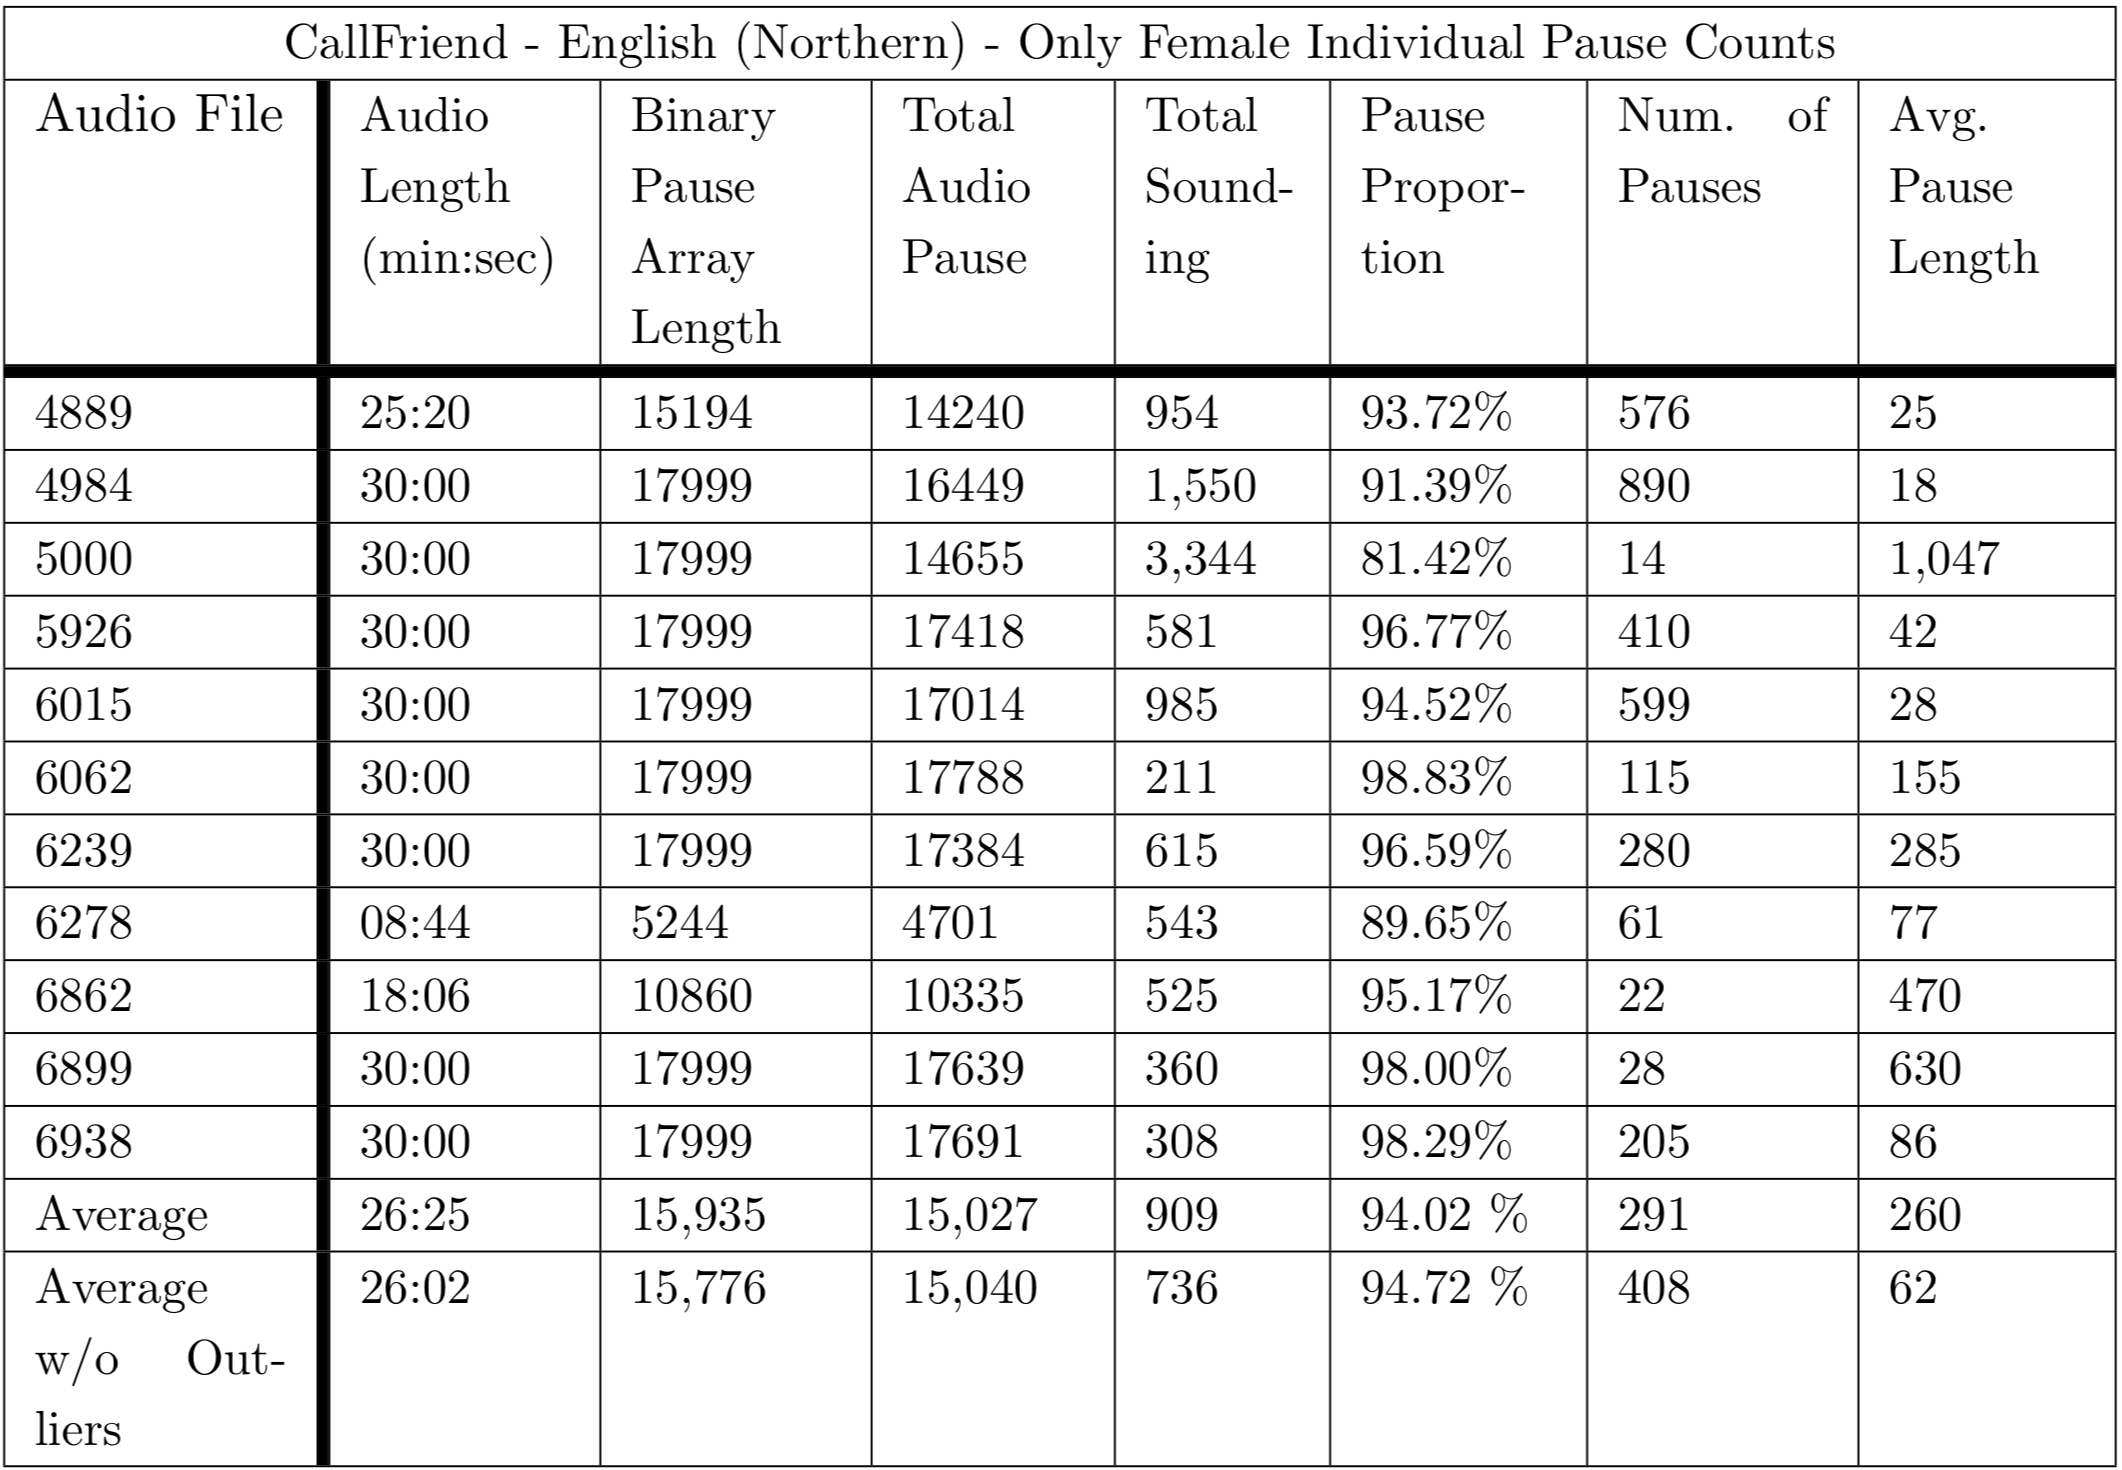
\includegraphics[scale=0.4]{src/main-matter/results/experiment-sex/pause-analysis/female-pause-table}
		\caption{Table 6.3: Only Female Audio Files and their Pause Usage, Outliers are 5000, 6062, 6239, 6862, 6899}
		\label{female-10bins}
	\end{center}
\end{figure}
\begin{figure}[h!]
	\begin{center}
		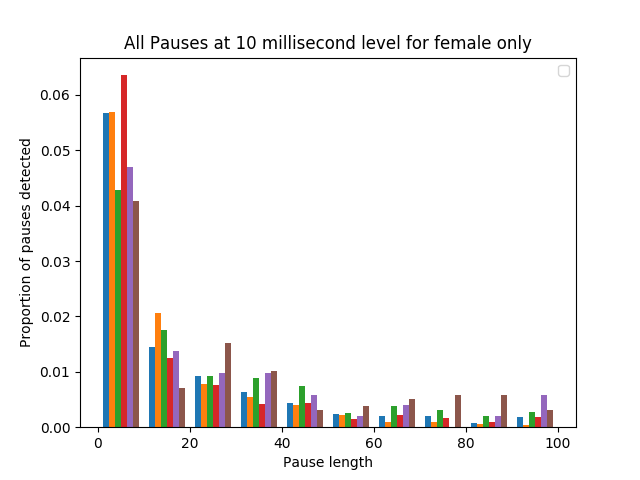
\includegraphics[scale=0.7]{src/main-matter/results/experiment-sex/pause-analysis/pause_histogram_bin10female}
		\caption{Histogram of All Pause Lengths per audio files 4889, 4984, 5926, 6015, 6278, 6938 - Female Only - Outliers removed}
		\label{female-10bins}
	\end{center}
%\end{figure}
%\begin{figure}[hb]
	\begin{center}
		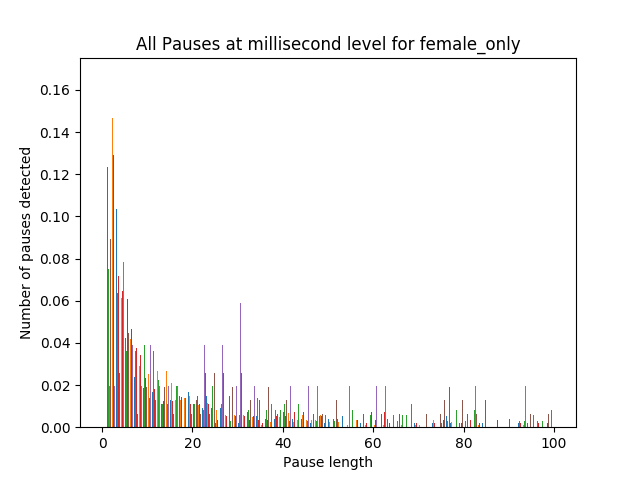
\includegraphics[scale=0.7]{src/main-matter/results/experiment-sex/pause-analysis/pause_histogram_bin100female}
		\caption{Histogram - All Pause Lengths per audio files 4889, 4984, 5926, 6015, 6278, 6938 - Female Only - Outliers removed}
		\label{default}
	\end{center}
\end{figure}








%From \ref{female-10bins} it can be seen that even though the audio files had different numbers of pauses digitised the same distribution was still seen throughout each file. This resembles the zipf mandlebrot li law. Based upon the data above, we can see an average of 400 pauses detected, this means if we want to get 20 data points in our entropy profile, we will have to either have windows of size 20 with no overlap, or allow overlap. if no overlap, this decreases the amount of symbols we should be aiming to include as having too many can throw off the estimation if not enough samples are collected initially in the window stage. if not enough sample are collected this could lead to false negative or false positive readings in terms of determining typical or atypical conversation. so choosing window sizes that a small in proportion to this is important as is choosing small symbol sets. \\



%\paragraph{To Do:\\}
%Update Table - include variance and mean into the data above, also change the data above because im pretty sure its wrong, use the values taken from the code. 
%? - Show the proportion of male to male vs female to female vs female to male. (So normalise the y axis)
%Mega Hist - Show the histogram of pauses lengths for each group
%Mega hist - Show the histogram of binary pauses for each group
%Mega chart - Show the probabilistic ranked symbol for each group and how one changes from the other
%? - Show the number of pauses of one group vs the other (so seeing what the normalisation took away)
%Bar Chart - Show pausing vs non-pausing in the files as an average \\
%Table - Compute the variance and mean of the rows above \\
%Plot - Do up a gaussian of the variance and mean outlined above \\
%Error - Shouldn't there be 1,800,000 pause length? I think theres that many milliseconds in a half an hour, not 18,000. Am I doing the time frame wrong? \\
%Error - Fix table ref not working
%Audio Files - Try redoing one of the shit audio files with a different frequency and see if that changes it. See if I can spot the times when the error occurs!
%Pause - Check the pause count is right, it seems far far too high to have 17788 out of 17999 be pauses for a conversation? Also sounds insane the other way around.
%Avg Pause Length - Take the avg from the freq array and put that into the table instead of the avg I did now. 
%Boxplot - Include boxplot
%include symbol sets 
%\afterpage{\clearpage}






%\subsubsection{\underline{Only Male Conversations}}
\begin{figure}[ht]
	\begin{center}
		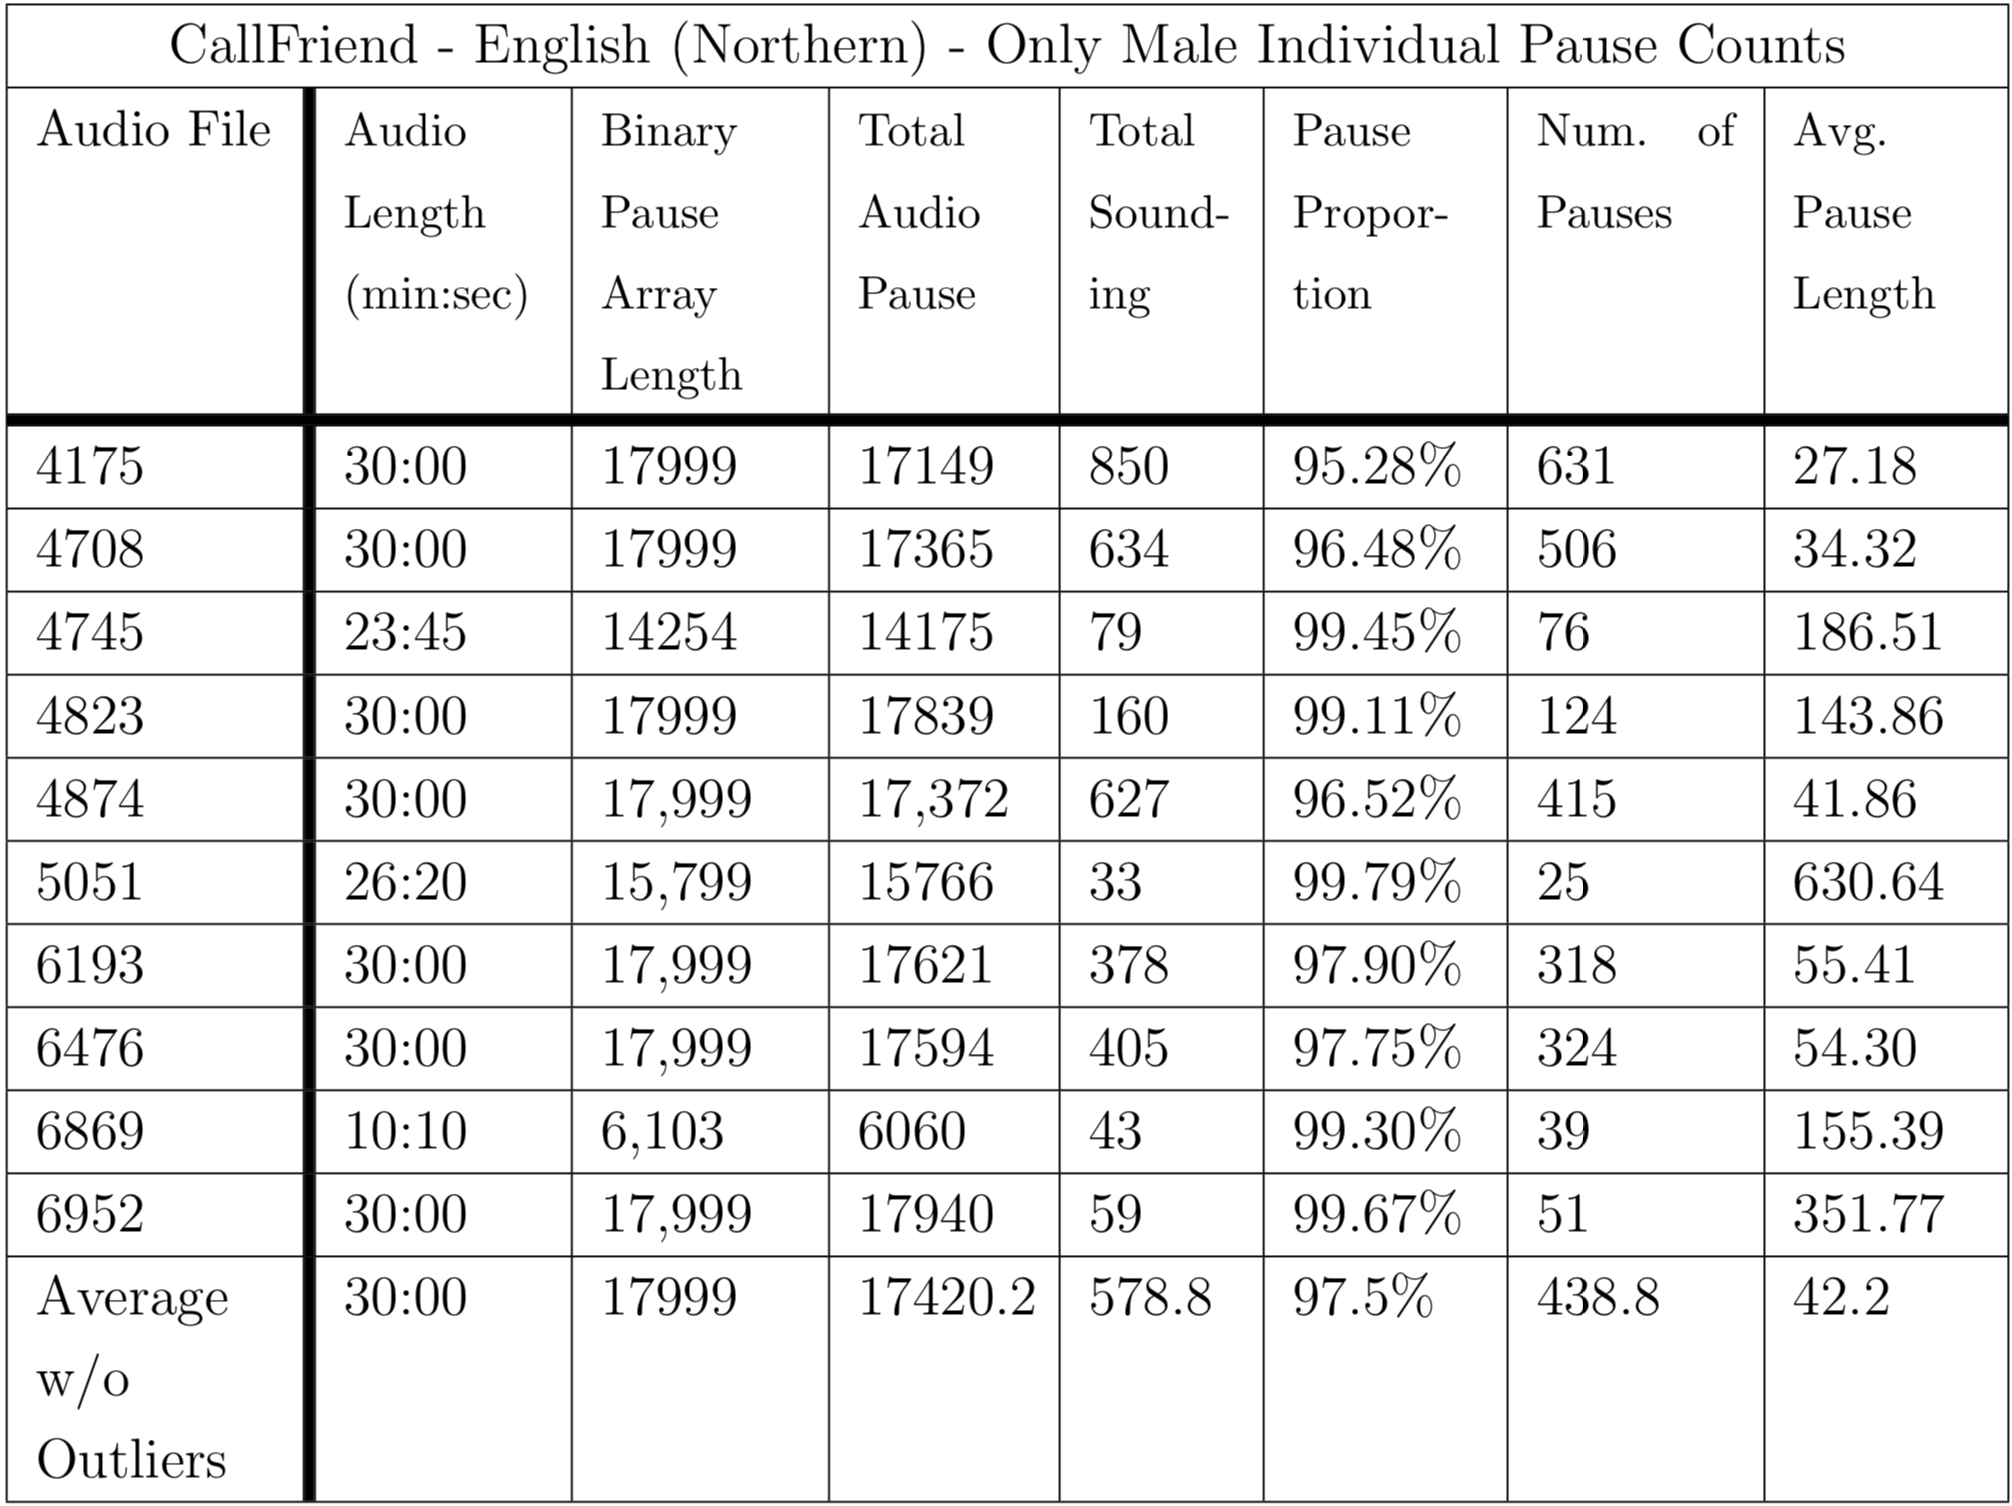
\includegraphics[scale=0.45]{src/main-matter/results/experiment-sex/pause-analysis/male-pause-table}
		\caption{Table 6.4: Only Male Audio Files and their Pause Usage, Outliers were 4745, 4823, 5051, 6869, 6952}
		\label{female-10bins}
	\end{center}
\end{figure}







%\begin{table}[h!]
%	\begin{tabular}{ | p{1.8cm} | | p{1.5cm} | p{1.5cm} | p{1.3cm} | p{1.1cm} | p{1.4cm} | p{1.5cm} | p {1.4cm} |}
%		\hline
%		\multicolumn{8}{| c |}{CallFriend - English (Northern) - Only Male Individual Pause Counts} \\%
%		\hline
%		{\small Audio File} & {\footnotesize Audio Length (min:sec)} &  {\footnotesize Binary Pause Array Length} & 
%			{\footnotesize Total Audio Pause} & {\footnotesize Total Sounding} & {\footnotesize Pause Proportion} & 
%			{\footnotesize Num. of Pauses} & {\footnotesize Avg. Pause Length} \\
%		\hline\hline
%		4175 & 30:00 & 17999 & 17149 & 850 & 95.28\% & 631 & 27.18 \\
%		\hline 
%		4708 & 30:00 & 17999 & 17365 & 634 & 96.48\% & 506 & 34.32 \\
%		\hline 
%%		\rowcolor{lightgray} 
%		4745 & 23:45 & 14254 & 14175 & 79 & 99.45\% & 76 & 186.51 \\
%		\hline 
%%		\rowcolor{lightgray} 
%		4823 & 30:00 & 17999 & 17839 & 160 & 99.11\% & 124 & 143.86 \\
%		\hline 
%		4874 & 30:00 & 17,999 & 17,372 & 627 & 96.52\% & 415 & 41.86 \\
%		\hline 
%%		\rowcolor{lightgray} 
%		5051 & 26:20 & 15,799 & 15766 & 33 & 99.79\% & 25 & 630.64 \\
%		\hline
%		6193 & 30:00 & 17,999 & 17621 & 378 & 97.90\% & 318 & 55.41 \\
%		\hline 
%		6476 & 30:00 & 17,999 & 17594 & 405 & 97.75\% & 324 & 54.30 \\
%		\hline 
%%		\rowcolor{pink} 
%		6869 & 10:10 & 6,103 & 6060 & 43 & 99.30\% & 39 & 155.39 \\
%		\hline 
%%		\rowcolor{lightgray} 
%		6952 & 30:00 & 17,999 & 17940 & 59 & 99.67\% & 51 & 351.77 \\
%		\hline 
%%		Average & xx:xx & 1x9 & 17x0 & sounding & --\% & 631 & avg  \\
%%		\hline
%		Average w/o Outliers & 30:00 & 17999 & 17420.2 & 578.8 & 97.5\% & 438.8 & 42.2  \\
%		\hline
%	\end{tabular}
%	\label{tab:sex-male}
%	\caption{Table: \ref{tab:sex-male} - Only Male Audio Files and their Pause Usage, Outliers were 4745, 4823, 5051, 6869, 6952} \\
%\end{table}









\afterpage{\clearpage}
%\subsubsection{\underline{Mixed Sex Conversations}}
\begin{figure}[h]
	\begin{center}
		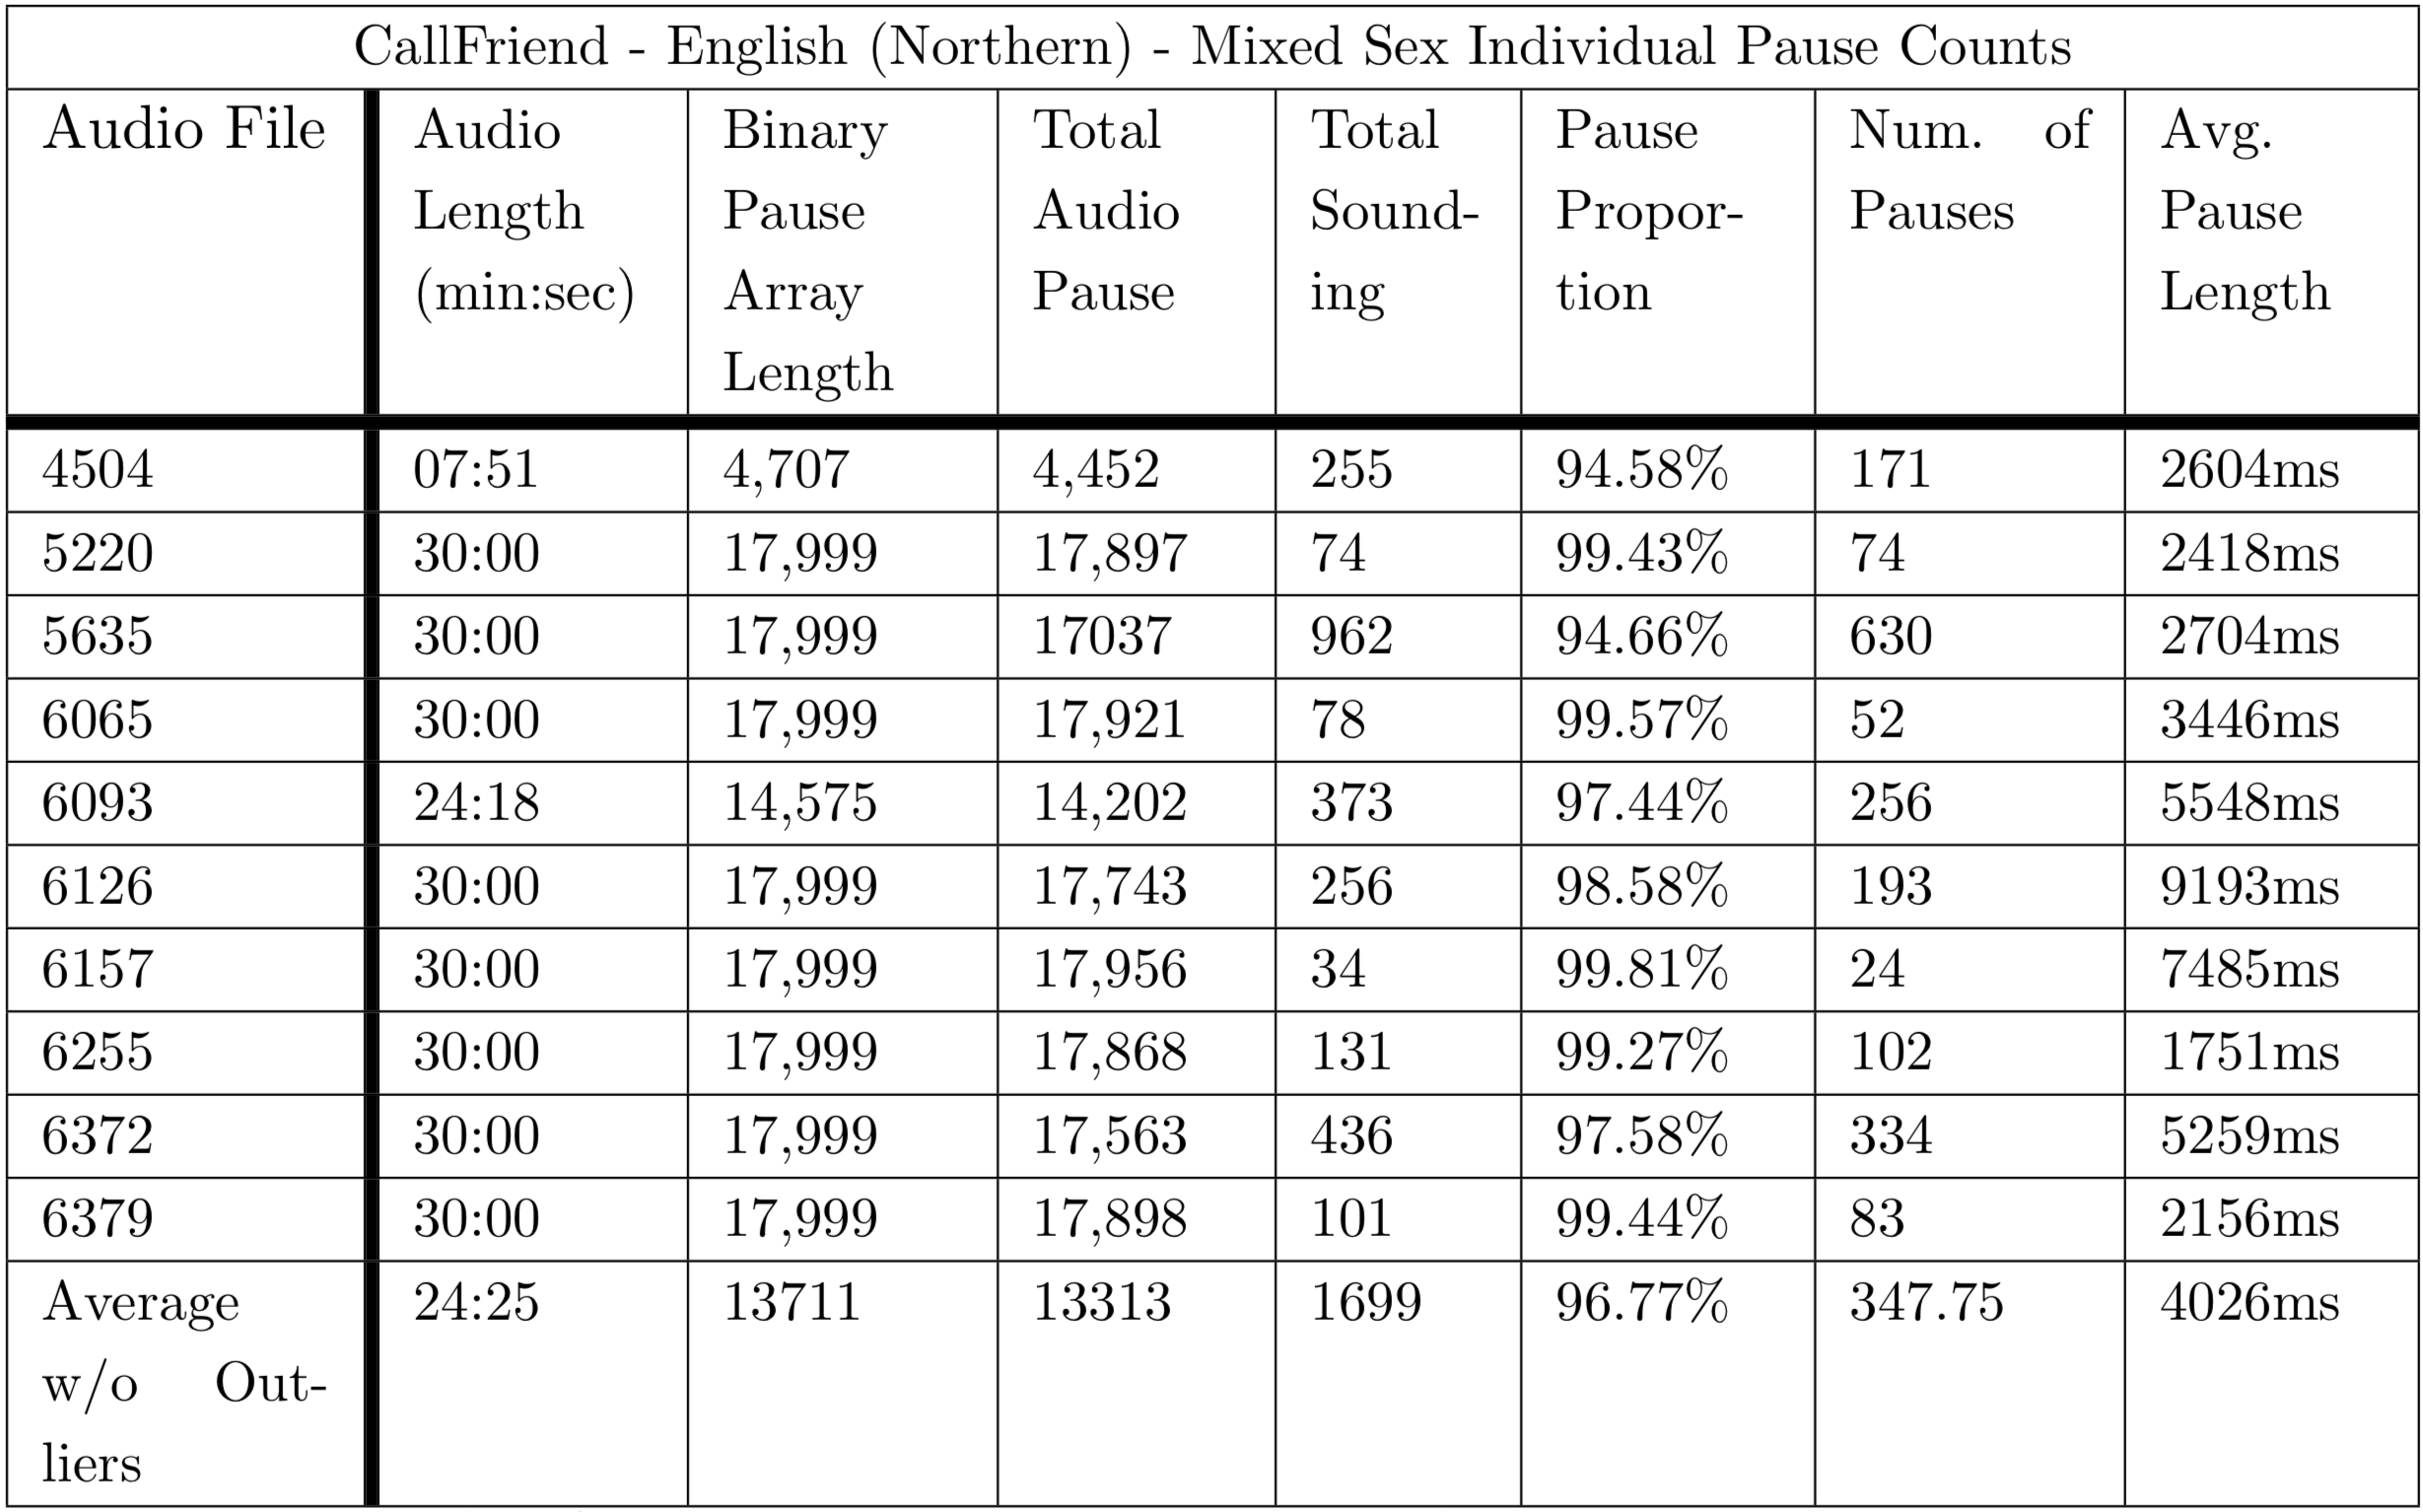
\includegraphics[scale=0.35]{src/main-matter/results/experiment-sex/pause-analysis/mixed-pause-table}
		\caption{Table 6.3: Mixed Sex Audio Files and their Pause Usage, Outliers were 5220, 6065, 6126, 6157, 6255, 6379}
		\label{female-10bins}
	\end{center}
\end{figure}









%	\begin{tabular}{ |p{1.8cm}| |p{1.5cm} |p{1.5cm} |p{1.3cm} |p{1.1cm} |p{1.4cm} |p{1.5cm} |p {1.4cm} |}
%		\hline
%		\multicolumn{8}{|c|}{CallFriend - English (Northern) - Mixed Sex Individual Pause Counts} \\%
%		\hline
%		{\small Audio File} & {\footnotesize Audio Length (min:sec)} &  {\footnotesize Binary Pause Array Length} & 
%			{\footnotesize Total Audio Pause} & {\footnotesize Total Sounding} & {\footnotesize Pause Proportion} & 
%			{\footnotesize Num. of Pauses} & {\footnotesize Avg. Pause Length} \\
%		\hline\hline
%		4504 & 07:51 & 4,707 & 4,452 & 255 & 94.58\% & 171 & 2604ms  \\
%		\hline 
%%		\rowcolor{lightgray} 
%		5220 & 30:00 & 17,999 & 17,897 & 74 & 99.43\% & 74 & 2418ms \\
%		\hline 
%		5635 & 30:00 & 17,999 & 17037 & 962 & 94.66\% & 630 & 2704ms \\
%		\hline 
%%		\rowcolor{lightgray} 
%		6065 & 30:00 & 17,999 & 17,921 & 78 & 99.57\% & 52 & 3446ms \\
%		\hline 
%		6093 & 24:18 & 14,575 & 14,202 & 373 & 97.44\% & 256 & 5548ms \\
%		\hline 
%%		\rowcoloe{lightgray}
%		6126 & 30:00 & 17,999 & 17,743 & 256 & 98.58\% & 193 & 9193ms \\
%		\hline 
%%		\rowcolor{lightgray} 
%		6157 & 30:00 & 17,999 & 17,956 & 34 & 99.81\% & 24 & 7485ms \\
%		\hline 
%%		\rowcolor{lightgray} 
%		6255 & 30:00 & 17,999 & 17,868 & 131 & 99.27\% & 102 & 1751ms \\
%		\hline 
%		6372 & 30:00 & 17,999 & 17,563 & 436 & 97.58\% & 334 & 5259ms \\
%		\hline 
%%		\rowcolor{lightgray} 
%		6379 & 30:00 & 17,999 & 17,898 & 101 & 99.44\% & 83 & 2156ms \\
%		\hline 
%%		Average & 27:22 & - & - & -&-&-& 197.4 \\
%%		\hline
%		Average w/o Outliers & 24:25 & 13711 & 13313 & 1699 & 96.77\% & 347.75 & 4026ms\\
%		\hline
%	\end{tabular}
%	\label{tab:1}
%	\caption{Table: \ref{tab:1} - Mixed Sex Audio Files and their Pause Usage, Outliers were 5220, 6065, 6126, 6157, 6255, 6379} \\


%\subsubsection{\underline{Comparisons}}
\begin{figure}[h]
	\begin{center}
		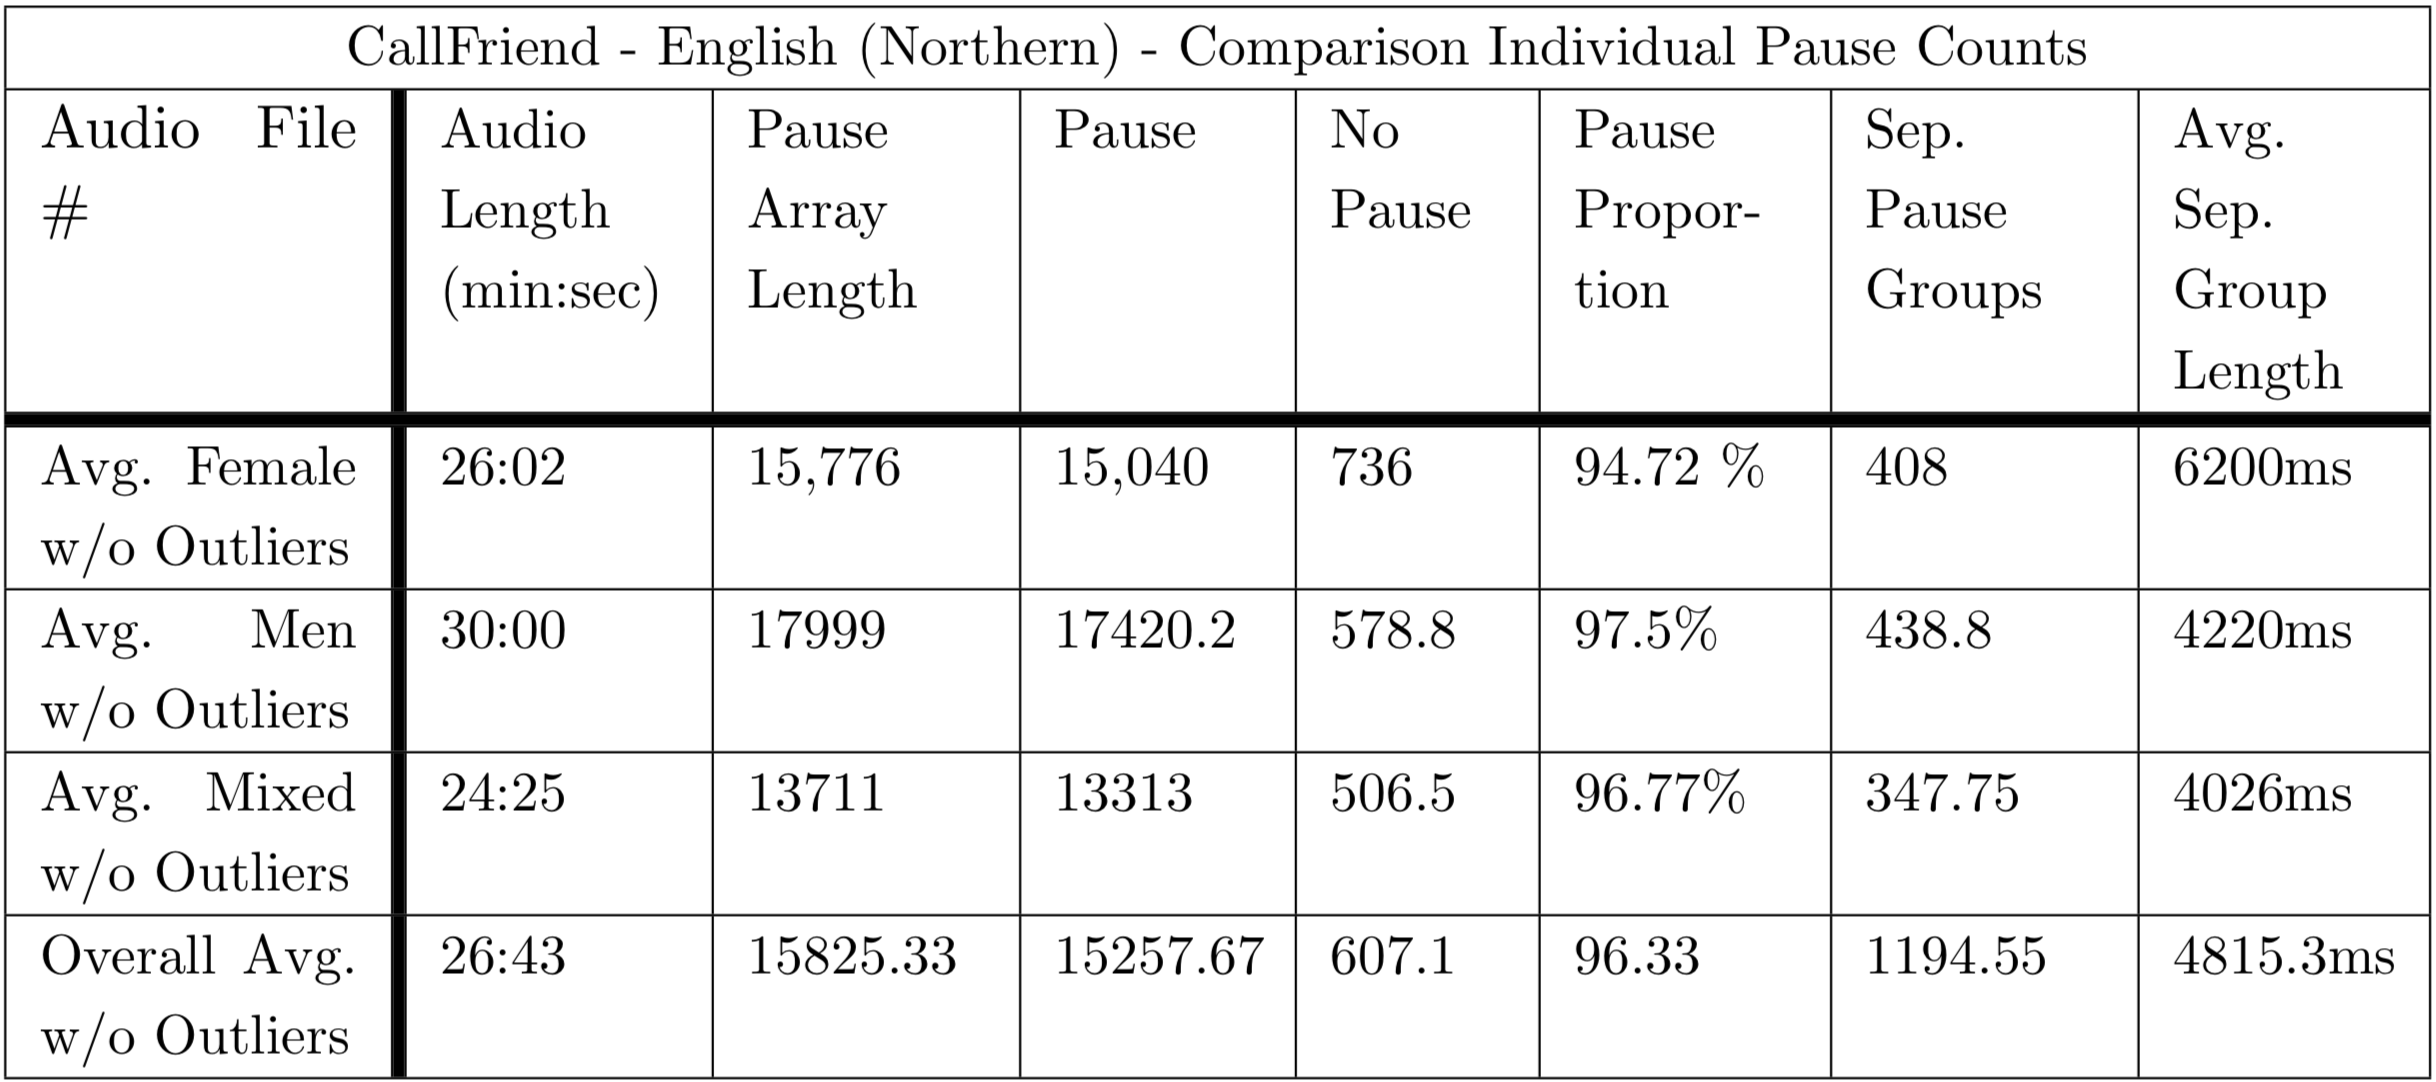
\includegraphics[scale=0.35]{src/main-matter/results/experiment-sex/pause-analysis/comparison-pause-table}
		\caption{Table 6.3: Comparison of sex based audio file pause analysis, Outliers were removed}
		\label{female-10bins}
	\end{center}
\end{figure}


%\begin{tabular}{ |p{2cm}| |p{1.5cm} |p{1.5cm} |p{1.3cm} |p{1.1cm} |p{1.4cm} |p{1.5cm} |p {1.4cm} |}
%		\hline
%		\multicolumn{8}{|c|}{CallFriend - English (Northern) - Comparison Individual Pause Counts} \\%
%		\hline
%		{\small Audio File \#} & {\footnotesize Audio Length (min:sec)} &  {\footnotesize Pause Array Length} & 
%			{\footnotesize Pause} & {\footnotesize No Pause} & {\footnotesize Pause Proportion} & {\footnotesize Sep. Pause Groups}  & {\footnotesize Avg. Sep. Group Length}\\
%		\hline\hline
%		Avg. Female w/o Outliers & 26:02  & 15,776 & 15,040 & 736 & 94.72 \% & 408 & 6200ms \\
%		\hline 
%		Avg. Men w/o Outliers & 30:00 & 17999 & 17420.2 & 578.8 & 97.5\% & 438.8 & 4220ms  \\
%		\hline 
%		Avg. Mixed w/o Outliers & 24:25 & 13711 & 13313 & 506.5 & 96.77\% & 347.75 & 4026ms\\
%		\hline
%		Overall Avg. w/o Outliers & 26:43 & 15825.33 & 15257.67 & 607.1 & 96.33 & 1194.55 & 4815.3ms \\
%		\hline
%	\end{tabular}
%	\label{tab:1}
%	\caption{Table: \ref{tab:1} - Average of each group Audio Files and their Pause Usage} \\

%\begin{figure}[h]
%	\begin{center}
%		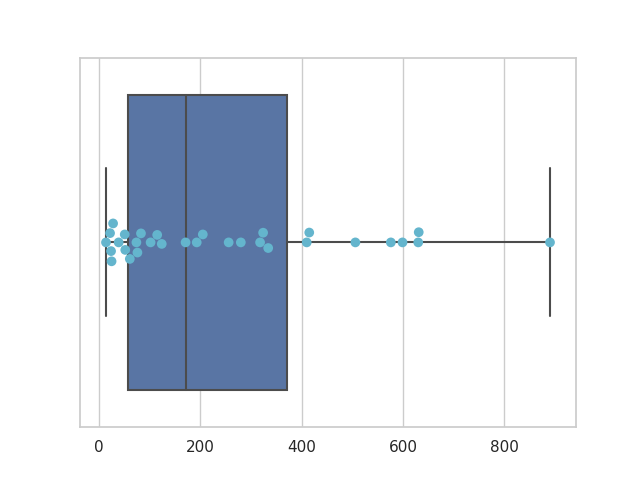
\includegraphics[scale=0.2]{src/main-matter/results/experiment1-sex/pause-analysis/pause_groups_num_all_whisker}
%		\caption{Average Pause Length per audio file - All Files - Outliers included - Whisker Plot}
%		\label{default}
%	\end{center}
%\end{figure}

%\subsubsection{Results}
%Due to the lack of results from the pause analysis, no symbol models were created.
%\paragraph{To Do:\\}
%Table - Show the averages of all groups together in a single table and see if theres any noticeable patterns or difference between them (e.g. male male vs female female)
%Age - Should I add the ages of the speakers as a column now and refer to them again in the next section, or just repeat the table with an extra column?
%Raincloud plot - show the raincloud plot here of all the different groups together. Could be interesting! 
%\begin{verbatim}https://mlwhiz.com/blog/2019/04/19/awesome_seaborn_visuals/\end{verbatim}
%\begin{verbatim}
%https://d212y8ha88k086.cloudfront.net/manuscripts/16574/49f87590-f903-4ad3-8d1b-096b518b4e2c_15191_-_rogier_kievit.pdf?doi=10.12688/wellcomeopenres.15191.1&numberOfBrowsableCollections=1&numberOfBrowsableGateways=9
%\end{verbatim}



%\subsection{Plots and data analysis}
%\subsubsection{Histograms}
%Show overlay of the bell curves of different number of pauses for all groups over the top of a single normal to show how they vary.
%
%Show all the rainclouds side by side?

